\chapter{Real time processing in the Big Data context [VI]}
\label{chap:real_time_processing}

Common paragraph

Web-companies encounter nowdays necessity to process data streams in the real-time fashion.
These streams produce often vast amount of data in a short period of time.
There are plenty of examples: Google's Zeitgeist system that tracks trends in search queries (some more examples\ldots)

There are many algorithms for processing data streams.
They divide to categories depending on what type of query do they answer.
A few query types are: ``has an item already been observed?'', ``how many times has an item been observed?'', ``what is the number of unique items among observed?'', etc.

How all this can be used in the speed layer

\section{Examples from real life}

Describe several examples how well-known companies apply real-time processing to the real data.
What algorithms do they maybe use, what topology or schema of computations in general.

\section{Stream processing algorithms}

To create aggregations, indicies and views of data, coming from the stream, we have often to answer different mathematical questions.
For example: ``has a particular item already been observed in the stream?'', ``how many times specific item has already arrived from the stream?'', ``what is the cardinality of the set of items so far observed in the stream?'', etc.
We can represent all these questions in a mathematical way, in the form of sets, values and functions.

To answer such questions stream processing algorithms, or \textit{sketch algorithms}\mnote{sketch algorithm}, exist.
They consider data coming from the stream as a mathematical space of values of a particular type, and compute functions on that space.
The result of those functions, a set of values, that gives an opportunity to answer particular query.

Sketch algorithm receives data from the stream and continuously builds the \textit{sketch}\mnote{sketch}.
Sketch is a data structure that persists only the part of information that stream produces.
It is always compact and stores not original values from the stream, but specific type of aggregation.

In comparison with the amount of original data, sketch algorithm uses small amount of memory to maintain sketch.
Sketch is usually a variation of hash-table or combination of several hash-tables.
It allows to answer particular query fast, mostly in a constant time, that does not depend on the size of the sketch.

Sketch algorithm produces usually only approximated result.
This is logical, because it condenses data set coming from the stream.
Technically speaking, it answers query with error that is the function of algorithm's parameters.
For example, if the answer to the query is a boolean answer (yes or no), wrong answer can occur with some probability.
If the answer is a number, deviation from exact right value is possible.

\subsection{Bloom filter}

The Bloom filter answers query ``has a particular item been observed in the stream?''
It works in a constant time and requires small amount of memory to hold.
It has several parameters that affect its size, time of request and rate of error.

The Bloom filter is essentially a hash-table, but it does not store elements themselves.
Instead, it is internally a bitset.
It uses several hash-functions, so that when we put new element into the Bloom filter, it computes hash-values using each hash-function, interpret them as indices, and put 1 by each of them.
To query an element, it does the same thing, it computes all hash-functions, and checks, whether all positions are equal to 1.
If so, the Bloom filter answers ``yes'', and it can be false positive, because hash-functions produce collisions.
We can adjust rate of false positives, changing parameters of the Bloom filter.
If answers is ``no'', it is always true by definition of the filter.
Figure~\ref{fig:bloom_filter} depicts the inner state and the way of requests to the Bloom filter.

\begin{figure}
  \centering
  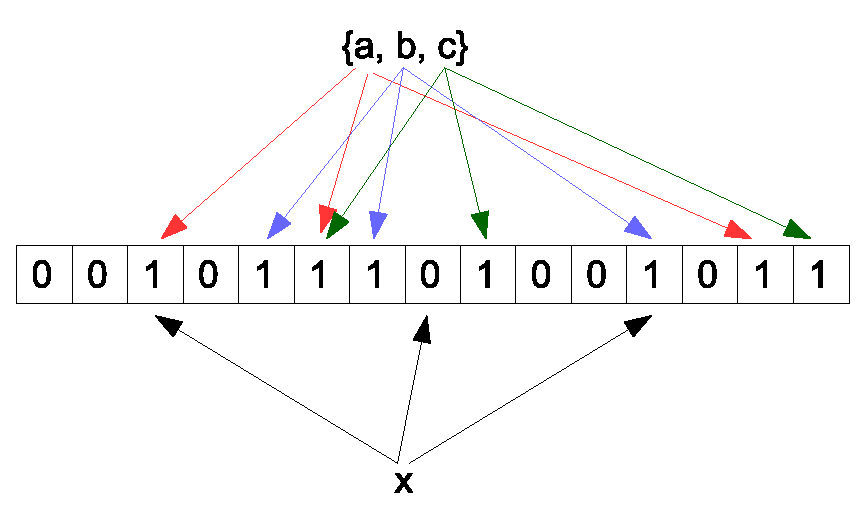
\includegraphics [width=0.6\textwidth]{images/BloomFilter}
  \caption{The inner state and requests to the Bloom filter.}
  \label{fig:bloom_filter}
\end{figure}

The Bloom filter has three parameters that affect its properties.
$m$ - the size of the filter, i.e. the number of bits in the bitset.
Its variation defines not only memory usage, but also the rate of false positives, because the more bits are in use, the less probability of collisions.
$k$ - the number of hash-functions.
This parameter influences again the rate of error.
If there are too less hash-functions, probability to encounter bits, set to 1 by other value, gets more.
At the same time, if there too many hash-functions, filter gets full faster, and again, probability to meet all 1 grows.
Also this parameter affects speed of request to the filter, because every additional hash-function requires time to compute.
$n$ - the number of values, already inserted into the filter.
This parameter is not inherent for the filter, but has a dynamic nature, because it depends on the statistical properties of the stream.
Nevertheless, it affects filter's behavior and is to consider.

Next expression describes the rate of false positives as a function of all three parameters discussed

$$
FP\_rate = \Bigg(1 - \Bigg[1 - \frac{1}{m}\Bigg]^{kn}\Bigg)^k \approx \Big(1 - e^{-kn/m}\Big)^k
$$

Having set parameters $m$ and $n$ we can infer the optimal number of hash-functions, that minimizes error rate

$$
k = \frac{m}{n}ln2
$$

Bloom filter is a great algorithm, that finds many examples of use.
Early UNIX spell-checkers used the Bloom filter to check spelling fast, prestoring the whole dictionary in the filter \cite{BroderMitzenmacher}.
The Bloom filter allows to store all unsuitable passwords, that users are not permitted to choose \cite{BroderMitzenmacher}.
Bitcoin uses the Bloom filter to speed up wallet synchronization (cite to online documentation!!!).
Google BigTable and Cassandra systems use the Bloom filter to reduce the number of hard disk lookups \cite{Bigtable/Chang_Dean_Ghemawat}.

\subsection{Count-min sketch}



\subsection{HyperLogLog algorithm}
\subsection{Flajolet-Martin sketch}

\section{Application in the speed Layer}

Descirbe how stream processing algorithms can be applied in the speed layer.
How can we build topology to solve some particular task, to creat some aggreagation for example.
How all this works technically, data pipelines, usage of different algorithms.